\documentclass[a4paper,11pt]{article}
%\usepackage{epsf}
\usepackage[latin1]{inputenc}
%\usepackage{graphicx}
%Check if we are compiling under latex or pdflatex
   \ifx\pdftexversion\undefined
     \usepackage[dvips]{graphicx}
   \else
     \usepackage[pdftex]{graphicx}
   \fi

\advance\textwidth by 60pt
\advance\textheight by 100pt
\advance\oddsidemargin by -25pt
\advance\evensidemargin by -25pt
\advance\topmargin by -50pt

\usepackage[colorlinks=true,urlcolor=blue]{hyperref}

%%%%%%%%%%%%%%%%%%%% stuff for graphics %%%%%%%%%%%%%%%%%%%%%

\usepackage{tikz}
%%%<
\usepackage{verbatim}
\usetikzlibrary{calc,trees,positioning,arrows,chains,shapes.geometric,%
    decorations.pathreplacing,decorations.pathmorphing,shapes,%
    matrix,shapes.symbols}

\tikzset{
>=stealth',
  punktchain/.style={
    rectangle, 
    rounded corners, 
    % fill=black!10,
    draw=black, very thick,
    text width=12em, 
    %text width=10em, 
    minimum height=3em, 
    text centered, 
    on chain},
  line/.style={draw, thick, <-},
  element/.style={
    tape,
    top color=white,
    bottom color=blue!50!black!60!,
    minimum width=8em,
    draw=blue!40!black!90, very thick,
    text width=10em, 
    minimum height=3.5em, 
    text centered, 
    on chain},
  every join/.style={->, thick,shorten >=1pt},
  decoration={brace},
  tuborg/.style={decorate},
  tubnode/.style={midway, right=2pt},
}

%%%%%%%%%%%%%%%%%%%%%%%%%%%%%%%%%%%%%%%%%%%%%%%%%%%%%%%%%%%%%%%%%%

\begin{document}

\newcommand{\etal}{{\it et al.}}
\newcommand{\DegN}{$^{\circ}$N}
\newcommand{\DegW}{$^{\circ}$W}
\newcommand{\DegE}{$^{\circ}$E}
\newcommand{\DegS}{$^{\circ}$S}
\newcommand{\Deg}{$^{\circ}$}
\newcommand{\DegC}{$^{\circ}$C}


\title{\textbf{User guide for DMONTOOLS}}  

\author{R. Dussin, J.M. Molines, J. Le Sommer \thanks{Laboratoire des Ecoulements Geophysiques et Industriels, CNRS UMR 5519, Grenoble, France} }


\date{September 2010}

\maketitle

%---------------------------------------------
\section{Introduction}

The Drakkar MONitoring TOOLS (hereafter DMONTOOLS) is a package to perform the monitoring of DRAKKAR simulations. It includes 
4 subpackages :




\begin{center}
\begin{figure}[!h]
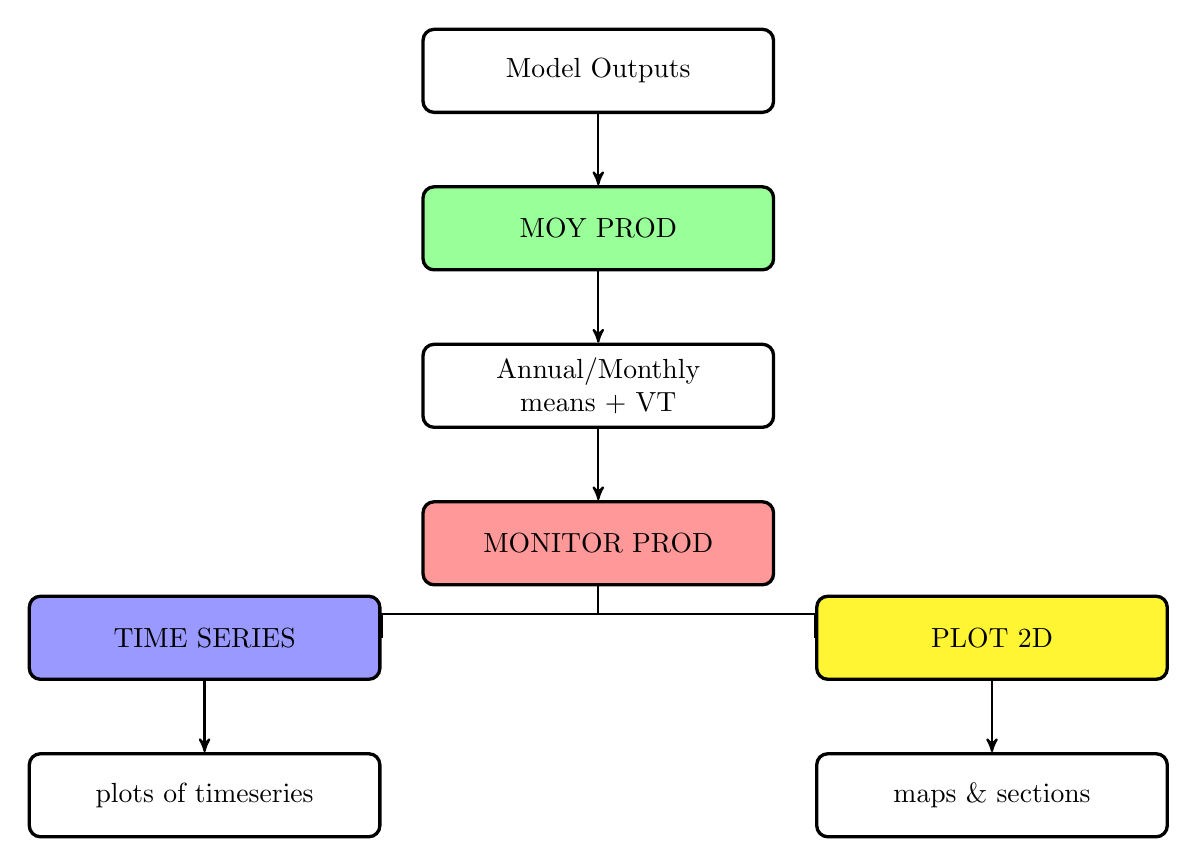
\begin{tikzpicture}
[node distance=1.2cm,
  start chain=going below,]

    \node [punktchain](modelout){Model Outputs};
	\node [punktchain, below of=modelout, node distance = 0.8cm, fill=green!40 ](cdftools){MOY PROD};
	\node [punktchain, below of=cdftools, node distance = 0.8cm](means){Annual/Monthly means + VT};
	\node [punktchain, below of=means, node distance = 0.8cm, fill=red!40 ](dmontools){MONITOR PROD};
	\node [punktchain, left of=dmontools, node distance = 5cm, fill=blue!40 ](timeseries){TIME SERIES};
	\node [punktchain, right of=dmontools, node distance = 5cm, fill=yellow!80 ](plot2d){PLOT 2D};
	\node [punktchain, below of=timeseries, node distance = 0.8cm](ts2){plots of timeseries};
	\node [punktchain, below of=plot2d, node distance = 0.8cm](plot2){maps \& sections};
	\draw[|-,-|,->, thick,] (modelout.south) |-+(0,-1em)-| (cdftools.north);
	\draw[|-,-|,->, thick,] (cdftools.south) |-+(0,-1em)-| (means.north);
	\draw[|-,-|,->, thick,] (means.south) |-+(0,-1em)-| (dmontools.north);
	\draw[|-,-|,-, thick,] (dmontools.south) |-+(0,-1em)-| (timeseries.east);
    \draw[|-,-|,-, thick,] (dmontools.south) |-+(0,-1em)-| (plot2d.west);   
    \draw[|-,-|,->, thick,] (timeseries.south) |-+(0,-1em)-| (ts2.north);   
    \draw[|-,-|,->, thick,] (plot2d.south) |-+(0,-1em)-| (plot2.north); 


\end{tikzpicture}
%\caption{}
\end{figure}
\end{center}

\begin{enumerate}
\item MOY\_PROD : Computes annual means and VT files
\item MONITOR\_PROD : Computes diagnostics on model outputs (usually annual or monthly means) and produces small netcdf
files which contains time-series of diagnosed quantities.
\item TIME\_SERIES : Creates the time-series diagrams  from the files created by MONITOR\_PROD.
\item PLOT\_2D : Produces selected maps or sections from model outputs. 
\end{enumerate}

\clearpage
\newpage

\section{Install}

\subsection{pre-requisites}

To use DMONTOOLS, you must already have some software already installed on your computer. The installation
of DMONTOOLS can be done without this software installed but it will fail at runtime. Here is what you need :

\begin{itemize}
\item standard linux software : image magick, gifsicle
\item NCAR Graphics Library $ \geq 5.1.1$ (available at \url{http://www.earthsystemgrid.org})
\item python packages : numpy, matplotlib and a netcdf interface (Scientific.IO, scipyIO, pynetcdf,...)
\item drakkar tools : cdftools, chart/coupe 
\end{itemize}

\subsection{step by step}

\noindent
In this section, we show how to install the DMONTOOLS package on ulam, choosing the WORKDIR as our root
directory. Adjust to your own machine and taste.


\begin{enumerate}

\item \textbf{Make sure you have your Drakkar Config Manager variables set :}

you will need PDIR and SDIR set in your .profile (PDIR is usually set to HOME directory and
SDIR to data directory)

\item \textbf{Checkout the package :}

\begin{verbatim}
svn co https://servforge.legi.grenoble-inp.fr/svn/DMONTOOLS/tags/1.0 DMONTOOLS
\end{verbatim}

\item \textbf{Run the installer :}

\begin{verbatim}
./install.ksh
\end{verbatim}

\noindent
the installer will ask you where to install python libs and bins
and will update PATH and PYTHONPATH in your shell environment.

\item \textbf{Optional - Compile the MPI\_TOOLS :}

\begin{verbatim}
cd $WORKDIR/DMONTOOLS/MPI_TOOLS
ln -s macro.ulam make.macro
gmake
\end{verbatim}

\end{enumerate}

\clearpage
\newpage

\section{Usage}

\subsection{Computing the Means and VT}

The MOY\_PROD subpackage allows to compute the means and VT in parallel jobs. It computes one year
at the time but split the computation onto 12 processors for means (one proc per month) and 12 more
processors for VT.
\\[0.2cm]
\par


\begin{enumerate}
\item  \textbf{mkmeans \textit{CONFIG CASE} :}

This command creates a RUN\_CONFIG/CONFIG\_CASE/CTL/CDF directory and copies the necessary
scripts for the means and VT computation.

\item \textbf{go to CDF directory and edit config\_moy.ksh :}

The config\_moy.ksh is your configuration file for your CONFIG CASE. Some informations are
filled automatically whereas some needs to be edited by hand. Pay attention to the
TYP\_LIST which must contains the file types you want to proceed.

\item \textbf{./RUN\_calmoy.ksh \textit{year}}

According to the batch manager defined in config\_moy.ksh, this script executes
RUN\_calmoy\_LoadLev.ksh or RUN\_calmoy\_PBS.ksh with the given year.

\end{enumerate}

\subsection{Doing the Monitoring}

The subpackages MONITOR\_PROD and PLOT\_2D also allow to do the monitoring in parallel jobs.
This time, each processor is dedicated to one particuliar year.
\\[0.2cm]
\par

\begin{enumerate}
\item \textbf{mkmonitor \textit{CONFIG CASE} :}

This command creates a RUN\_CONFIG/CONFIG\_CASE/CTL/CDF directory and copies the necessary
scripts for the monitoring.

\item \textbf{go to CDF directory and edit config\_def.ksh :}

The config\_def.ksh is your configuration file for your CONFIG CASE. Some informations are
filled automatically whereas some needs to be edited by hand. It contains the menus for monitor prod,
plot 2D et time series.

\item \textbf{./RUN\_metamon.ksh \textit{year1 year2}}

This script will submit the MONITOR\_PROD part of the DMONTOOLS. It takes two years as arguments. When we are working in parallel
(useMPI = 1) we can compute a set of several years (depending on the machine) at once. The arguments are then the first and last year
of the set of years you want to compute in the job. In a serial job, only the first arguement is used (give anything as year2).
This produces a set of small netcdf and text files stored in CONFCASE-DIAGS on the storage machine.

\item \textbf{./make\_ncdf\_timeseries.ksh \textit{CONFIG CASE YEAR0} :}

This produces concatenated netcdf from those computed by MONITOR\_PROD and stores them in CONFCASE-MONITOR. 
YEAR0 must be the starting year of the run, not the first year of the monitoring.
Those netcdf files are ready to be processed by the TIME\_SERIES subpackage.

\item \textbf{./run\_monitor\_py :}

This script will plot the timeseries from the netcdf stored in CONFCASE-MONITOR. 

\item \textbf{./RUN\_plot\_monitor.ksh \textit{year1 year2}}

This script will submit the PLOT\_2D part of the DMONTOOLS. Same remarks about arguments.
It produces cgm files in the PLOTS directory.

\item \textbf{./make\_movies.ksh :}

This script produces animated gif from the cgm files in the PLOTS directory. There is also a version for tracers
(\textit{make\_movies\_trc.ksh}). Those jobs can be submitted to the batch manager.

\end{enumerate}

\clearpage
\newpage

\section{Contribute to DMONTOOLS :}

\begin{itemize}

\item \textbf{How to create new time-series ?}

To create new time-series, you have to modify files in \textbf{bin}, \textbf{MONITOR\_PROD} and \textbf{TIME\_SERIES}.

In \textbf{bin}, add your new flags (which allows the other users to use your diag or not) in \textit{config\_def.ksh}. 
If you have written advanced shell functions that could be used by other diags, you should add them in the "common functions" 
section of \textit{function\_def.ksh}.

In \textbf{MONITOR\_PROD}, the core of the production process is \textit{monitor\_prod.ksh}. This is where you add
the computation of your diags.
The results must be saved in netcdf yearly files (use ncrcat to concatenate if needed). The filename has
to give explicitely the config, case and year. Those files will be stored in the DIAGS/NC directory.
Then, you have to modify \textit{make\_ncdf\_timeseries.ksh} to create a concatenated netcdf from all the yearly files.
In this step, you can also merge several netcdf files if you want to reduce the number of resulting files.
The idea is to gather the information and reduce the number of input files for the plotting scripts.

In \textbf{TIME\_SERIES}, add your python scripts for plotting the results in the lib directory. You are advised
to copy one of the example.py script as a template. Your scripts have to contain read, plot and save functions.
Finally, update \textit{run\_moni\-tor\_py.ksh} (in \textbf{TIME\_SERIES/scripts}) and 
\textit{run\_moni\-tor\_py\_stand\-alone.ksh} (in \textbf{bin}) so that they read the new flags.

Hereafter is a summary of the different steps (white is for \textbf{bin}, red is for \textbf{MONITOR\_PROD} and blue for
\textbf{TIME\_SERIES}).

\begin{center}
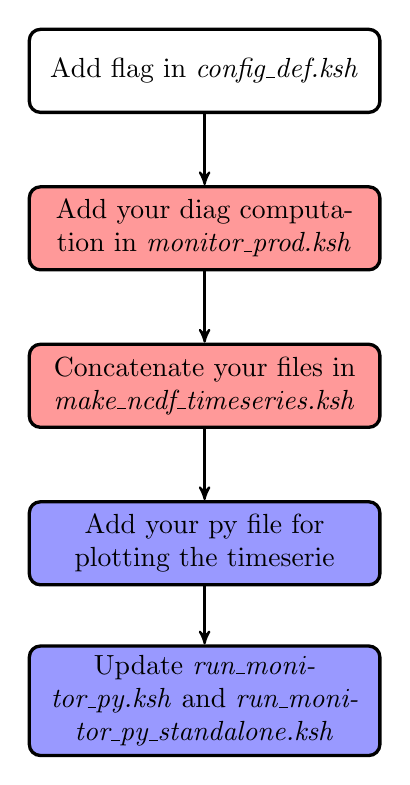
\begin{tikzpicture}
[node distance=.8cm,
  start chain=going below,]

    \node [punktchain](flag){Add flag in \textit{config\_def.ksh}};
	\node [punktchain, below of=flag, node distance = 1.2cm, fill=red!40 ](monprod){Add your diag computation in \textit{monitor\_prod.ksh}};
	\node [punktchain, below of=monprod, node distance = 1.2cm, fill=red!40](makenc){Concatenate your files in
	                                                                                 \textit{make\_ncdf\_timeseries.ksh}};
	\node [punktchain, below of=makenc, node distance = 1.2cm, fill=blue!40 ](createpy){Add your py file for plotting the timeserie};
	\node [punktchain, below of=createpy, node distance = 1.2cm, fill=blue!40 ](monpy){Update \textit{run\_moni\-tor\_py.ksh} and 
	                                                                   \textit{run\_moni\-tor\_py\_stand\-alone.ksh}};
	\draw[|-,-|,->, thick,] (flag.south) |-+(0,-1em)-| (monprod.north);
	\draw[|-,-|,->, thick,] (monprod.south) |-+(0,-1em)-| (makenc.north);
	\draw[|-,-|,->, thick,] (makenc.south) |-+(0,-1em)-| (createpy.north);
	\draw[|-,-|,->, thick,] (createpy.south) |-+(0,-1em)-| (monpy.north);

\end{tikzpicture}
\end{center}

\clearpage
\newpage

\item \textbf{How to create a new section or a new map ?}

To create a new time-serie, you have to modify files in \textbf{bin} and \textbf{PLOT\_2D}.

In \textbf{bin}, add your new flags (which allows the other users to use your diag or not) in \textit{config\_def.ksh}. 

In \textbf{PLOT\_2D}, the core of the production process is \textit{plot\_monitor.ksh}. This is where you add
the computation of your new maps or sections (using chart and coupe). The results are stored in cgm files. 
You can choose to send them to an existing storage subdirectory such as GLOBAL, OVT,... or in a new one.
If you choose to create a new subdirectory, you will also have to modify \textit{make\_movies.ksh} 
(or \textit{make\_movies\_trc.ksh} for tracers) to include this new directory to the list. 

Hereafter is a summary of the different steps (white is for \textbf{bin}, yellow is for
\textbf{PLOT\_2D}).

\begin{center}
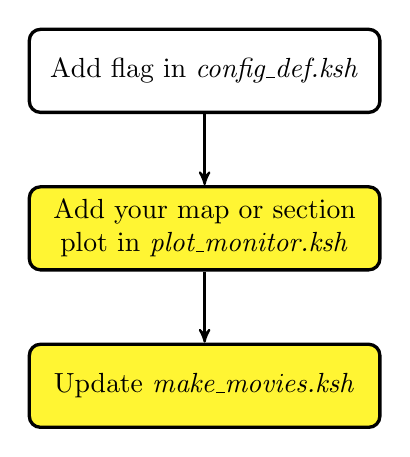
\begin{tikzpicture}
[node distance=.8cm,
  start chain=going below,]

    \node [punktchain](flag){Add flag in \textit{config\_def.ksh}};
	\node [punktchain, below of=flag, node distance = 1.2cm, fill=yellow!80 ](plotmon)
	                                                        {Add your map or section plot in \textit{plot\_monitor.ksh}};
	\node [punktchain, below of=plotmon, node distance = 1.2cm, fill=yellow!80](makets){Update
	                                                                                 \textit{make\_movies.ksh}};
	\draw[|-,-|,->, thick,] (flag.south) |-+(0,-1em)-| (plotmon.north);
	\draw[|-,-|,->, thick,] (plotmon.south) |-+(0,-1em)-| (makets.north);


\end{tikzpicture}
\end{center}

\end{itemize}

\clearpage
\newpage

\section{FAQ :}

\begin{itemize}
\item \textbf{Can I run the DMONTOOLS on a standard linux machine ?}

Yes ! Be sure you have your Drakkar environement variables (SDIR, PDIR,...) set, then Choose machine = desktop

\item \textbf{I have got ANNUAL in my annual means, will it work ?}

No ! But in MONITOR\_PROD/utils you have \textit{links\_annual\_files.ksh} which will fix this.

\item \textbf{What is the nomenclature for Levitus climatologies ?}

Levitus\_p2.1\_1y\_TS\_config.nc (for example : Levitus\_p2.1\_1y\_TS\_orca246.nc)

\item \textbf{My machine has a small number of cores, can I run multiple jobs at once ?}

Yes ! but only if your are on a machine with a batch manager that can create a volatile TMPDIR for the job
(example : ulam). Then set RNDTMPDIR = 1 and launch as many jobs as needed. 

\item \textbf{What is run\_monitor\_py\_standalone.ksh ?}

This is script is for those who already have all their netcdf files computed on machine A and only want to
perform the python part of the monitoring on machine B (generally because python is not installed on machine A).

\item \textbf{What if I run a climatlogical run ?}

The correct way to run the scripts is :

\textbf{./RUN\_meta\-mon.ksh 1 4} 

\textbf{./RUN\_plot\_moni\-tor.ksh 1 4}.

DO NOT put zeros before (e.g. \textbf{./RUN\_metamon.ksh 0001 0004} is the WRONG way to do it).

\item \textbf{What if I have interannual means ?}

The PLOT\_2D part is compatible with interannual means (for example 2000-2005) provided
you run it with useMPI=0 and do not run the \textit{make\_movies.ksh} (likely not to work).
It is also advised to put $create\_gif = 1$ to convert cgm files to gif.
The correct call is \textit{./RUN\_plot\_monitor.ksh 1997-2007 1} (second argument is unused but must be given)
The MONITOR\_PROD has not been tested.


\end{itemize}

\end{document}
